\documentclass[listof=nochaptergap]{report}

\usepackage[utf8]{inputenc}
\usepackage[english]{babel}
\usepackage{geometry}
\usepackage{graphicx}
\usepackage{hyperref}
\usepackage{tikz}
\usepackage{pgfplots}
\usepackage{listings}
\usepackage{minted}
\usepackage{caption}
\usepackage{setspace}

\geometry{
    paper=a4paper,
    top=32mm,
    bottom=32mm,
    left=25mm,
    right=25mm
}

\setminted[cpp]{
    frame=lines,
    framesep=2mm,
    fontsize=\footnotesize,
    linenos,
    breaklines
}

\renewcommand{\lstlistingname}{Algorithm}% Listing -> Algorithm
\renewcommand{\lstlistlistingname}{List of \lstlistingname s}% List of Listings -> List of Algorithms



\begin{document}
    \begin{titlepage}
        \noindent
        
\includegraphics[width=1.0\textwidth]{images/Q04_HTW_Berlin_Logo_quer_pos_FARBIG_RGB.jpg}


        \vspace{2cm}

        \begin{center}
            \noindent
            \huge{\textbf{Grayscale, RGB to HSV and Emboss parallelized with OpenMP}}

            \vspace{1cm}

            \noindent
            \LARGE{Module: Programmierkonzepte und Algorithmen}

            \vspace{1cm}

            \noindent
            \small{\today}
        \end{center}

        \vfill

        \noindent
        \begin{minipage}[t]{0.5\textwidth}
            \begin{flushleft}
                \textbf{Student}\\
                Name: Christoph Stach\\
                Matrikel-Nr: 0555912                
            \end{flushleft}
        \end{minipage}
        \begin{minipage}[t]{0.5\textwidth}
            \begin{flushright}
                \textbf{Dozent}\\
                Mykyta Kovalenko\\
            \end{flushright}
        \end{minipage}
    \end{titlepage}

    \tableofcontents

    \chapter{Introduction}

This document includes the technical documentation about various task implemented with OpenMP. The goal of this document is to show the outcomes of various algorithms and compare their performance with the OpenCV library. OpenMP is a library that enables easy to use parallel computing on multiple CPUs. To demonstrate its capabilities the author implemented a Grayscale-, a RGB2HSV- and an Emboss-Algorithm. All of them consist of two For-Loops, which loop over all pixels of an image.\\

The run time of each algorithm was measured with different usage scenarios of OpenMP. To parallelize a program into multiple threads, OpenMP offers the \mintinline{cpp}{#pragma omp parallel for} compiler directive for For-Loops.  The author used OpenMP on the outer For-Loop, the inner For-Loop and both For-Loops. The results are shown in the following performance test diagrams for each algorithm. Also the results, the algorithms produce, are demonstrated and the implementation is given accordingly.\\

All performances tests were done on a Dell XPS 15 9955, with a Intel Core i7, 16GB ram and a nVidia GeForce GTX 960m.\\

The source code this document is based on is hosted on \url{http://github.com} under the \url{http://github.com/christophstach/openmp-emboss}.


    
    
    \chapter{Grayscale}


    \section{Performance Tests}

    \begin{center}
        \begin{figure}[H]
            \centering

            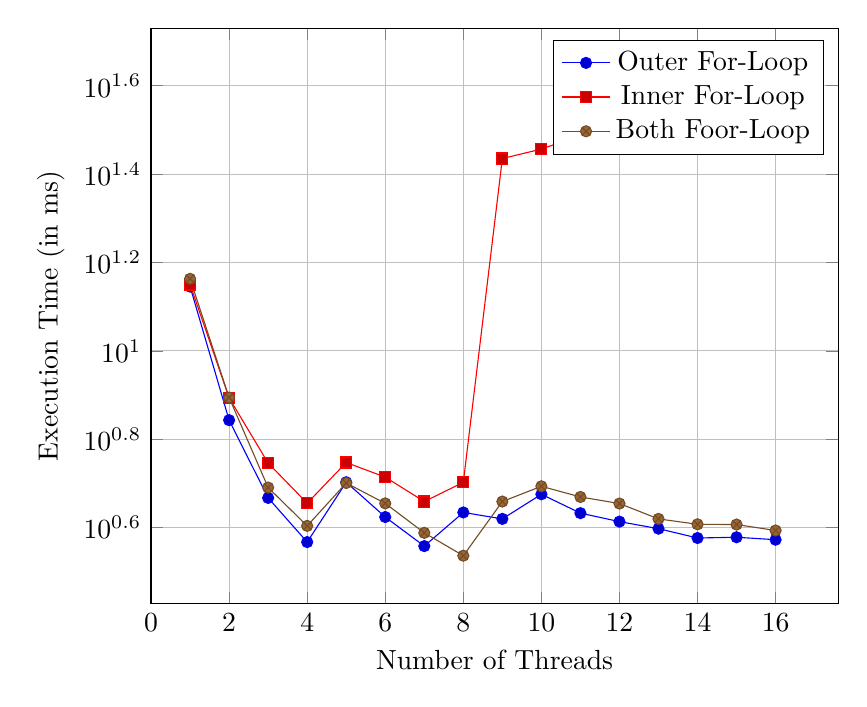
\begin{tikzpicture}
                \begin{axis}[
                    title={},
                    width=0.85\textwidth,
                    xlabel={Number of Threads},
                    ylabel={Execution Time (in ms)},
                    xmin=0,
                    ymin=0,
                    ymode=log,
                    grid=major
                ]
                    \addplot coordinates {
                        (1,13.9745)(2,6.96595)(3,4.6442)(4,3.68995)(5,5.03995)(6,4.20395)(7,3.61295)(8,4.3057)(9,4.1637)(10,4.7335)(11,4.28995)(12,4.10465)(13,3.9569)(14,3.76905)(15,3.7839)(16,3.7353)
                    };
                    \addlegendentry{Outer For-Loop}

                    \addplot coordinates {
                        (1,14.1323)(2,7.823)(3,5.5688)(4,4.5187)(5,5.58615)(6,5.1761)(7,4.5574)(8,5.0374)(9,27.2378)(10,28.6125)(11,30.7489)(12,33.5384)(13,35.3871)(14,36.3363)(15,39.2266)(16,41.8422)
                    };
                    \addlegendentry{Inner For-Loop}       

                    \addplot coordinates {
                        (1,14.5495)(2,7.8367)(3,4.9025)(4,4.01435)(5,5.0195)(6,4.5141)(7,3.8719)(8,3.4367)(9,4.55745)(10,4.93435)(11,4.66755)(12,4.50995)(13,4.16325)(14,4.048)(15,4.0425)(16,3.9195)
                    };
                    \addlegendentry{Both Foor-Loop}
                \end{axis}
            \end{tikzpicture}
            \caption{Grayscale Performance Tests}
        \end{figure}
    \end{center}

    \section{Results}

    \begin{figure}[H]
        \centering

        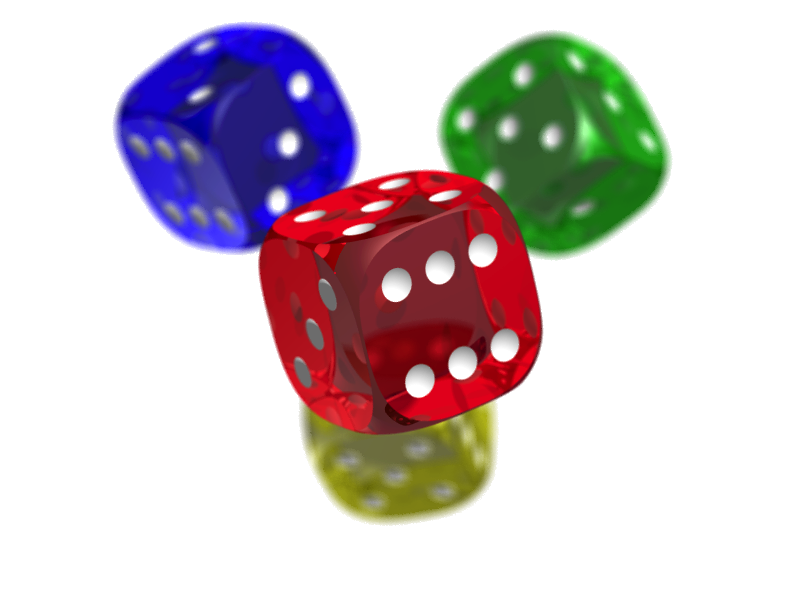
\includegraphics[width=0.25\textwidth]{images/dice.png}
        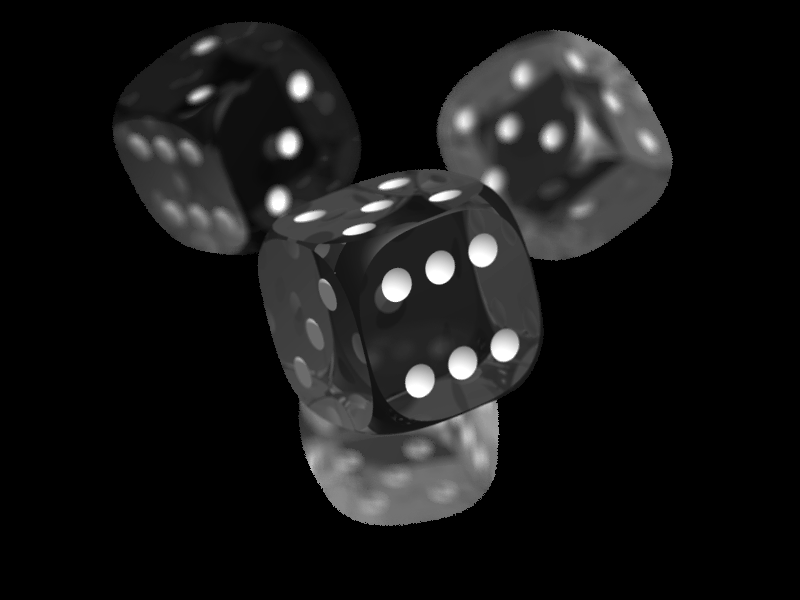
\includegraphics[width=0.25\textwidth]{images/cv-grayscale.png}
        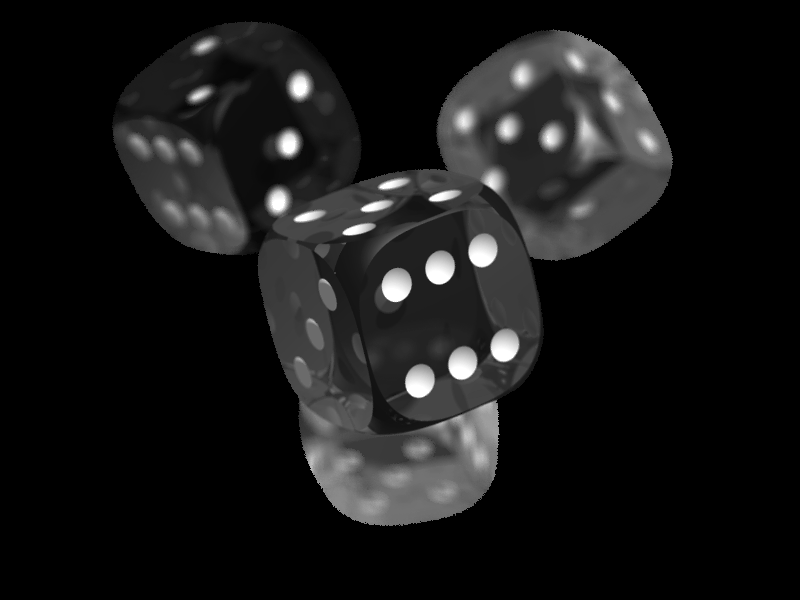
\includegraphics[width=0.25\textwidth]{images/own-grayscale.png}
        
        \caption{Grayscale results of OpenCV (middle) and self-implemented  Algorithm (right)}
        \label{fig:grayscale}
    \end{figure}


    \section{Implementation}

    

    \begin{listing}[H]
        \begin{minted}{cpp}
cv::Mat applyGrayscaleOuter(cv::Mat srcImage, int numThreads = omp_get_num_procs()) {
    auto destImage = cv::Mat(srcImage.rows, srcImage.cols, CV_8UC1);

    omp_set_num_threads(numThreads);

    #pragma omp parallel for default(none) shared(srcImage, destImage)
    for (int row = 0; row < srcImage.rows; row++) {
        for (int col = 0; col < srcImage.cols; col++) {
            auto srcPixel = srcImage.at<cv::Vec3b>(row, col);

            uchar r = srcPixel[2];
            uchar g = srcPixel[1];
            uchar b = srcPixel[0];

            // uchar destPixel = 0.21 * r + 0.72 * g + 0.07 * b; // luminosity formular
            uchar destPixel = 0.299 * r + 0.587 * g + 0.114 * b; // open cv formular

            destImage.at<uchar>(row, col) = destPixel;
        }
    }

    return destImage;
}
        \end{minted}
        \captionof{lstlisting}{Grayscale with parallelization of the outer For-Loop}
        \label{listing:grayscale}
    \end{listing}


\section{Comparison with OpenCV}

\subsection{Code}

\begin{listing}[H]
    \begin{minted}{cpp}
cv::Mat applyOpenCvGrayscale(const cv::Mat &srcImage) {
    cv::Mat destImage;
    cv::cvtColor(srcImage, destImage, cv::COLOR_BGR2GRAY);

    return destImage;
}
    \end{minted}
    \captionof{lstlisting}{Grayscale with OpenCV}
    \label{listing:grayscale_opencv}
\end{listing}

\subsection{Performance}


    \chapter{HSV}

HSV (Hue, Saturation, Value) is a different representation von the RGB (Red, Green, Blue) color-model. It is used to make easy adjustments according to it's components. Usually image programs and \LaTeX interpret images as RGB images. This is a reason for the colorful representation of the images.

\section{Performance Tests}

The RGB2HSV performance is also the best with a parallelization on the outer For-Loop. Strongly improving until the usage of 4 threads. Using 8 threads yields the performance peak. Same observations like in performance tests of \ref{fig:grayscale} were made when to many threads are in use.

\begin{center}
    \begin{figure}[H]
        \centering

        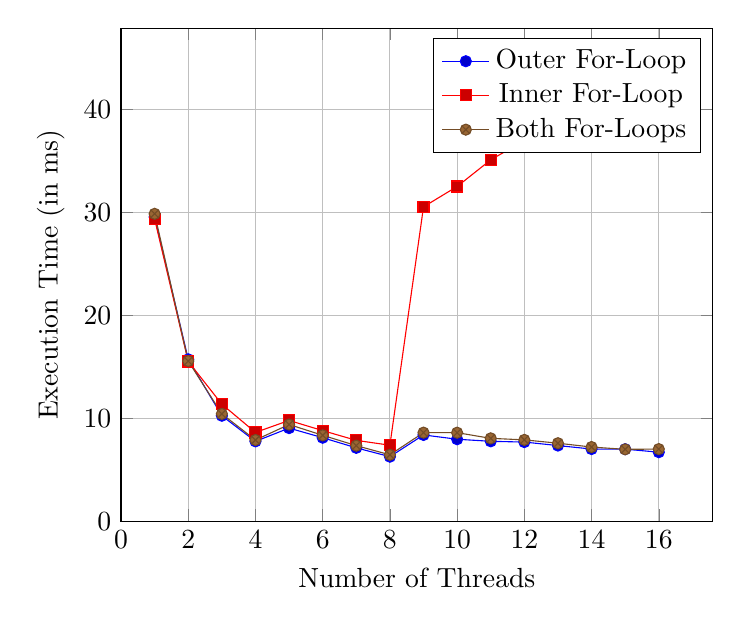
\begin{tikzpicture}
            \begin{axis}[
                title={},
                width=0.75\textwidth,
                xlabel={Number of Threads},
                ylabel={Execution Time (in ms)},
                xmin=0,
                ymin=0,
                grid=major
            ]
                \addplot coordinates {
                    (1,29.5366)(2,15.7231)(3,10.2453)(4,7.7598)(5,9.04545)(6,8.11285)(7,7.1297)(8,6.27195)(9,8.3824)(10,7.96645)(11,7.7646)(12,7.69085)(13,7.35195)(14,7.01335)(15,7.00095)(16,6.70895)
                };
                \addlegendentry{Outer For-Loop}

                \addplot coordinates {
                    (1,29.3423)(2,15.5132)(3,11.3651)(4,8.62715)(5,9.78995)(6,8.8026)(7,7.857)(8,7.38445)(9,30.5217)(10,32.4977)(11,35.0829)(12,36.9657)(13,37.1315)(14,39.4836)(15,39.4552)(16,43.51)
                };
                \addlegendentry{Inner For-Loop}
                
                \addplot coordinates {
                    (1,29.8459)(2,15.5525)(3,10.4249)(4,7.89)(5,9.39475)(6,8.3478)(7,7.3445)(8,6.45355)(9,8.6068)(10,8.60125)(11,8.05395)(12,7.9041)(13,7.581)(14,7.2079)(15,6.9847)(16,7.01045)
                };
                \addlegendentry{Both For-Loops}   
            \end{axis}
        \end{tikzpicture}
        \caption{RGB to HSV Performance Tests}
    \end{figure}
\end{center}

\section{Results}

The self-implemented algorithm yields very similar results compared to the OpenCV version. Subtracting the image matrices reveals a small differences, which could be the consequences of rounding-errors.

\begin{figure}[H]
    \centering

    \includegraphiThe self-implemented algorithm yields very similar results compared to the OpenCV version. Subtracting the image matrices reveals a small differences, which could be the consequences of rounding-errors.cs[width=0.20\textwidth]{images/dice.png}
    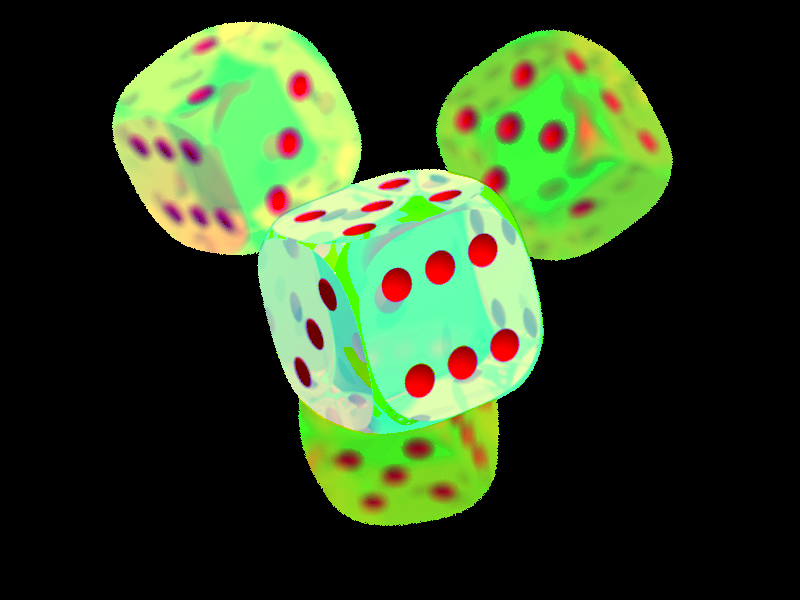
\includegraphics[width=0.20\textwidth]{images/cv-hsv.png}
    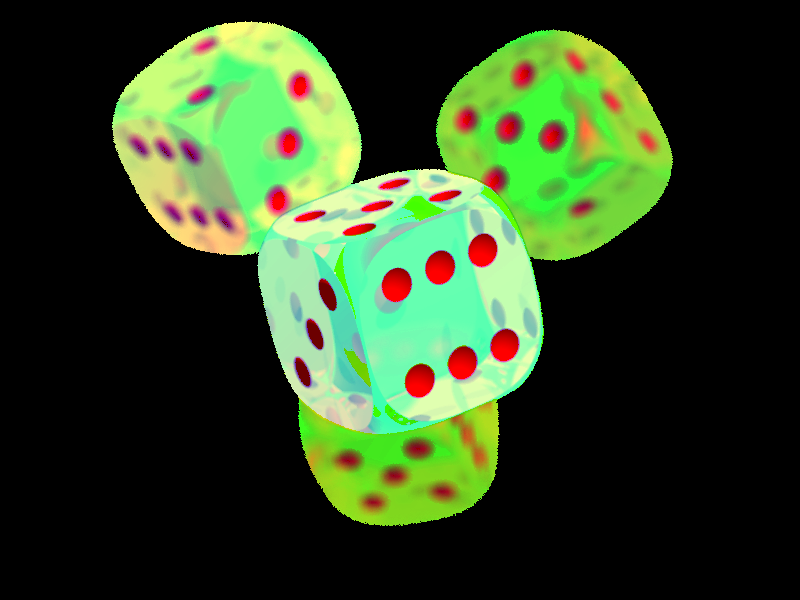
\includegraphics[width=0.20\textwidth]{images/own-hsv.png}
    
    \caption{RGB to HSV results of OpenCV (middle) and self-implemented  Algorithm (right)}
    \label{fig:hsv}
\end{figure}

\section{Implementation}

\begin{listing}[H]
    \begin{minted}{cpp}
cv::Mat applyHsvOuter(cv::Mat srcImage, int numThreads = omp_get_num_procs()) {
    cv::Mat destImage(srcImage.rows, srcImage.cols, CV_8UC3);
    omp_set_num_threads(numThreads);

    #pragma omp parallel for default(none) shared(srcImage, destImage)
    for (int row = 0; row < srcImage.rows; row++) {
        for (int col = 0; col < srcImage.cols; col++) {
            auto srcPixel = srcImage.at<cv::Vec3b>(row, col);

            double r = srcPixel[2] / 255.0;
            double g = srcPixel[1] / 255.0;
            double b = srcPixel[0] / 255.0;

            double h, s, v;

            double cMax = std::max(std::max(r, g), b);
            double cMin = std::min(std::min(r, g), b);
            double diff = cMax - cMin;

            if (cMax == cMin) {
                h = 0;
            } else if (cMax == r) {
                h = int(60 * ((g - b) / diff) + 360) % 360;
            } else if (cMax == g) {
                h = int(60 * ((b - r) / diff) + 120) % 360;
            } else {
                h = int(60 * ((r - g) / diff) + 240) % 360;
            }

            s = cMax == 0 ? 0 : (diff / cMax);
            v = cMax;

            cv::Vec3b destPixel = cv::Vec3b(
                    uchar(h / 360.0 * 180.0),
                    uchar(s * 255.0),
                    uchar(v * 255.0)
            );

            destImage.at<cv::Vec3b>(row, col) = destPixel;
        }
    }

    return destImage;
}
    \end{minted}
    \captionof{lstlisting}{RGB to HSV conversion with parallelization of the outer For-Loop}
    \label{listing:hsv}
\end{listing}

\section{Comparison with OpenCV}

\subsection{Code}


\begin{listing}[H]
    \begin{minted}{cpp}
cv::Mat applyOpenCvHsv(const cv::Mat &srcImage) {
    cv::Mat destImage;
    cv::cvtColor(srcImage, destImage, cv::COLOR_BGR2HSV);
    return destImage;
}
    \end{minted}
    \captionof{lstlisting}{RGB to HSV conversion  with OpenCV}
    \label{listing:hsv_opencv}
\end{listing}

\subsection{Performance}

OpenCV outperforms the self-implemented version significantly with a runtime of $ xxx $.
    \chapter{Emboss}

\section{Performance Tests}

\begin{center}
    \begin{figure}[H]
        \centering
        
        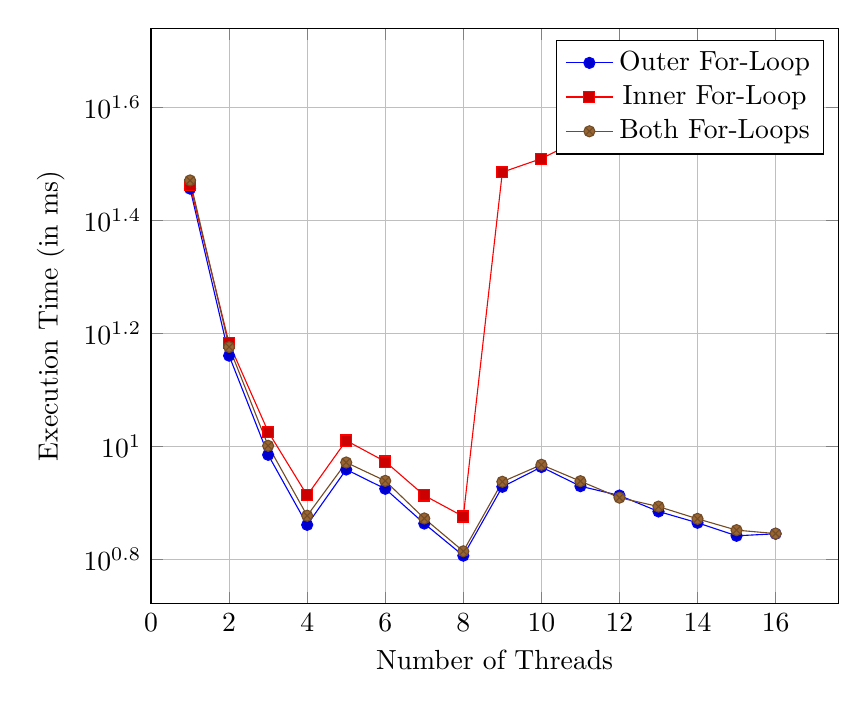
\begin{tikzpicture}
            \begin{axis}[
                title={},
                width=0.85\textwidth,
                xlabel={Number of Threads},
                ylabel={Execution Time (in ms)},
                xmin=0,
                ymin=0,
                ymode=log,
                grid=major
            ]
                \addplot coordinates {
                    (1,28.5583)(2,14.4724)(3,9.66625)(4,7.2702)(5,9.1055)(6,8.4178)(7,7.30745)(8,6.41185)(9,8.48695)(10,9.19905)(11,8.508)(12,8.1918)(13,7.677)(14,7.33135)(15,6.95245)(16,7.0099)
                };
                \addlegendentry{Outer For-Loop}

                \addplot coordinates {
                    (1,28.9709)(2,15.213)(3,10.6239)(4,8.1958)(5,10.2444)(6,9.4047)(7,8.1935)(8,7.52165)(9,30.54)(10,32.2743)(11,34.9379)(12,35.3693)(13,37.9348)(14,39.7072)(15,41.118)(16,45.1394)
                };
                \addlegendentry{Inner For-Loop}

                \addplot coordinates {
                    (1,29.5323)(2,14.9916)(3,10.0283)(4,7.545)(5,9.3703)(6,8.69475)(7,7.4621)(8,6.5289)(9,8.66325)(10,9.2846)(11,8.6837)(12,8.11935)(13,7.8319)(14,7.4501)(15,7.115)(16,7.01605)
                };
                \addlegendentry{Both For-Loops}
            \end{axis}
        \end{tikzpicture}
    \caption{Emboss Performance Tests}
    \end{figure}
\end{center}

\section{Results}

\begin{figure}[H]
    \centering

    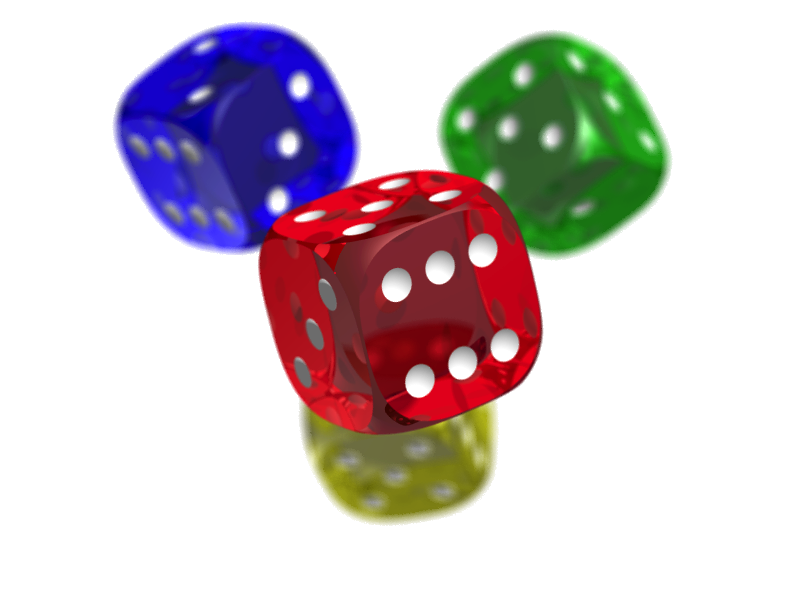
\includegraphics[width=0.25\textwidth]{images/dice.png}
    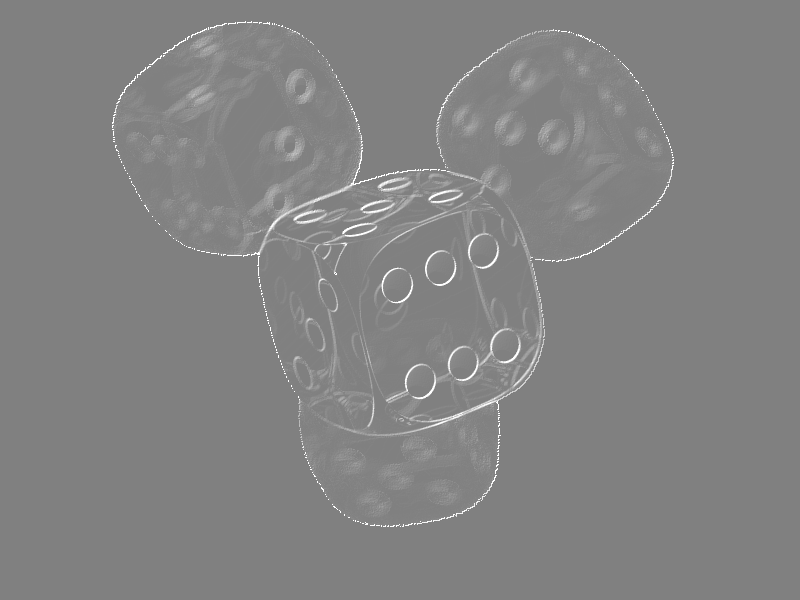
\includegraphics[width=0.25\textwidth]{images/own-emboss.png}
    
    \caption{Results of self-implemented Emboss-Algorithm}
    \label{fig:emboss}
\end{figure}

\section{Implementation}

\begin{listing}[H]
    \begin{minted}{cpp}
cv::Mat applyEmbossOuter(cv::Mat srcImage, int numThreads = omp_get_num_procs()) {
    cv::Mat destImage(srcImage.rows, srcImage.cols, CV_8UC1);
    omp_set_num_threads(numThreads);

    #pragma omp parallel for default(none) shared(srcImage, destImage)
    for (int row = 0; row < srcImage.rows; row++) {
        for (int col = 0; col < srcImage.cols; col++) {
            int diffR, diffG, diffB, diff, gray;
            auto srcPixel = srcImage.at<cv::Vec3b>(row, col);

            if (row == 0 || col == 0) {
                diffR = srcPixel[2];
                diffG = srcPixel[1];
                diffB = srcPixel[0];
            } else {
                auto upperLeftPixel = srcImage.at<cv::Vec3b>(row - 1, col - 1);
                diffR = std::abs(srcPixel[2] - upperLeftPixel[2]);
                diffG = std::abs(srcPixel[1] - upperLeftPixel[1]);
                diffB = std::abs(srcPixel[0] - upperLeftPixel[0]);
            }

            diff = std::max(diffR, std::max(diffG, diffB));

            gray = 128 + diff;
            gray = gray > 255 ? 255 : gray;
            gray = gray < 0 ? 0 : gray;

            destImage.at<uchar>(row, col) = gray;
        }
    }

    return destImage;
}
    \end{minted}
    \captionof{lstlisting}{Emboss with parallelization of the outer For-Loop}
    \label{listing:emboss}
\end{listing}

\section{Comparison with OpenCV}

OpenCV doesn't provide an implementation on the Emboss-Algorithm.
    

    \chapter{Conclusion}


    \begin{spacing}{1.0}
        \phantomsection
        \addcontentsline{toc}{chapter}{\listfigurename}
        \listoffigures        
    \end{spacing} 

    \begin{spacing}{1.75}
        \phantomsection
        \addcontentsline{toc}{chapter}{\lstlistlistingname}
        \lstlistoflistings        
    \end{spacing}
\end{document}